\documentclass[12pt, a4pape]{article}
\usepackage[utf8]{inputenc}
\usepackage{fancyhdr}
\usepackage{multicol}
\usepackage[russian]{babel}
\usepackage{amsmath}
\usepackage{amssymb}
\usepackage[a4paper, margin=1in]{geometry}
\usepackage{graphicx}%Вставка картинок правильная
\usepackage{float}%"Плавающие" картинки
\usepackage{wrapfig}%Обтекание фигур (таблиц, картинок и прочего)
\usepackage[usenames]{color}
\usepackage{array}
\pagestyle{fancy}
\fancyhf{} % Очистка всех полей заголовков

\setlength{\columnsep}{29pt}
\pagecolor[rgb]{1,1,1}
\geometry{
  a4paper,
  top=8mm, 
  right=16mm, 
  bottom=20mm, 
  left=8mm
}
\begin{document}
\newpage
\fancyfoot[R]{\thepage} 
\pagecolor[rgb]{1,1,1}
\begin{center}
\Large Федеральное государственное автономное образовательное учреждение высшего образования\\ «Национальный исследовательский университет ИТМО»\\
Факультет Программной Инженерии и Компьютерной Техники\\
\hfill 


\vspace{7cm}
\Large Лабораторная работа №6 \\
Работа с системой компьютерной вёрстки \TeX\\
Вариант: 2\\
\end{center}

\vspace{7.5cm}
 
\begin{flushright}
\textit{Выполнил:}\\
Ахроров Кароматуллохон Фирдавсович\\
Группа P3110\

\textit{Проверил:}\\
Практик по предмету информатика:\\
Рыбаков Степан Дмитриевич\\
\end{flushright}
 
\vfill

\begin{center} Санкт-Петербург, 2024 \end{center}


\newpage
\fancyfoot[R]{\thepage} 
\pagecolor[rgb]{1,1,1}
\begin{multicols}{3}
\footnotesize
\\ и отдельных недостатков. Не все указания можно признать удачными; некоторые из них представляют собой не совет, как искать решение, а сжатый план всего решения, и если план понятен, то остается провести лишь очевидные вычисления. Во многих случаях более уместно было бы задать читателю наводящий вопрос, а не рекомендовать сразу «рассмотреть то-то» или «поступать так-то».

\\В предисловии авторы пишут, что теоретические введения, которые предпосланы главам задачника, «нужно либо прочесть от начала до конца, либо не читать вовсе». К сожалению, во многих случаях юному читателю лучше рекомендовать второе. Введения же к некоторым главам (например, 7, 9, 23) совсем неудачны, ибо там сообщаются отрывочные сведения, часто дискуссионные и не соответствующие материалу стабильных учебников.

\\Можно отметить и ряд других дефектов. Решения к некоторым задачам приведены не самые лучшие. Например, задачу 6.10 проще решать «в лоб», следуя правилу умножения многозначного числа на однозначное; решение задачи 13.13 сильно сокращается, если проанализировать её условие и заметить, что для всех допустимых x должно выполняться неравенство c05 x>0. Встречаются в книге неточности и опечатки. Так, ответ к задаче 18.13 должен быть такой: 120-90 2 ки; в приводимом решении задачи существенно, что точки A и C, вокруг которых производится поворот, — вершины острых углов треугольника (очень рекомендуем читателю разобраться, где в решении это явно использовано). Условие задачи 12.7 неточно сформулировано — надо дополнительно предположить, что аB + BA = 0.

\\Впрочем, едва ли имеет смысл приводить здесь полный перечень отдельных недостатков. Молодой читатель, будем надеяться, понимает, что создание книги — дело довольно сложное, и не всегда удается избежать ошибок, несмотря на усилия авторов, все сделать идеально уже в первом издании. Подавляющее большинство включенных в книгу задач взято авторами из вариантов письменных работ, предлагавшихся в разные годы на вступительных экзаменах по математике в Московском университете, а также в ряде других вузов Москвы. Очень хорошо, что эти задачи, снабженные указаниями и решениями, становятся доступными широким массам любителей математики, входят в школьную практику. Но при этом было бы уместно точно указывать источник заимствования, поскольку эти задачи являются плодом коллективного творчества экзаменационных комиссий. Каждый, кто хоть раз занимался составлением задач, знает, скольких трудов и какого времени требует появление новой оригинальной задачи. Кстати, эти ссылки были бы полезны и читателю — он смог бы по ним составить представление об уровне требований, предъявляемых к поступающим в различные вузы или на разные факультеты университетов.\\Известный американский математик Д. Пойа в своей книге «Как решать задачу», посвященной общей методике решения математических задач, писал: «Если он (преподаватель математики) будет пробуждать любознательность учащихся, предлагая им задачи, соразмерные с их знаниями, и своими наводящими вопросами будет помогать им решать эти задачи, то он сможет привить им вкус к самостоятельному мышлению и развить необходимые для этого способности». Приятно представить и порекомендовать читателю книгу именно такого характера, книгу, имеющую своей целью не только показать, как решать задачи, но и подсказать (там, где это необходимо), как их решать.
\columnbreak
\subsection*{ВВЕДЕНИЕ \\В ЭЛЕКТРОНИКУ}

\\Выпущенная издательством МГУ книга кандидата
физико-математических наук А. М. Хазена «Введение в электронику» адресована школьникам, которые интересуются физикой, математикой и особенно электроникой и радиотехникой.
\\Книга рассчитана на массового читателя и вместе с тем написана на хорошем физическом уровне. Ясность изложения, оригинальность приведенных примеров сочетаются в ней с достаточной строгостью. Можно с уверенностью сказать, что для школьника, прочитавшего внимательно эту книгу, многие понятия электроники станут ясными.
\\Юным читателям будет
интересно узнать, что принцип обычного вакуумного диода может использоваться для создания генератора электрического тока, работающего за счет внешнего источника тепла, чем похожи и чем отличаются линейный ускоритель электронов и лампа бегущей волны, что такое взрывомагнитный генератор и тд.
\\ В книге выделяются узловые вопросы для различных классов электронных уст-
ройств. Несмотря на большое количество описанных в книга конкретных приборов, она не перегружена примерами.
\\ Книгу можно рекомендовать как пособие для школьников, выбравших технические дисциплины или физику своей будущей специальностью.

\vfill % Заполнение колонки до конца страницы
\end{multicols}
\hfill \textit{Н. Х. Розов \hspace{2cm} Д. Я. Сев.}
\vspace{1cm}

\newpage
\begin{figure}[H]

\centering

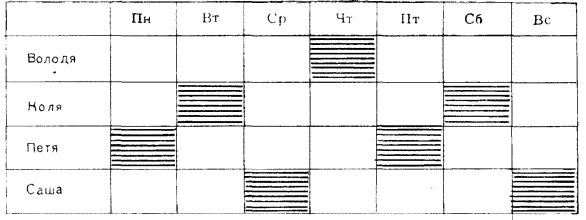
\includegraphics[width=1\linewidth]{lab6/image.png}

\label{fig:mpr}

\end{figure}

\[
(\left[\frac{2}{2}\right] + 1)^2 = 4 > \left[\frac{4}{2}\right] + 1 = 3. \hspace{0.4cm}
\]

% \begin{tabular}{l c c c c ccccc}
% \hline
% x $r$ & f1 & f2 & f3 & f4 & \\
% \hline
% A $r$ & $A$ & $B$ & $A$ & $B$ & $A$ & $B$ \\
% \hline
% B & A & $A$ & $B$ & $B$ & $A$  \\ 
% \hline

\begin{table}
    \centering
    \begin{tabular}{ccccc}
        x & f1 & f2 & f3 & f4 \\ \hline
        A & A & B & A & B \\ \hline
        B & A & A & B & B \\
    \end{tabular}
    \caption{Caption}
    \label{tab:my_label}
\end{table}

\\Выпущенная издательством МГУ книга кандидата
физико-математических наук А. М. Хазена «Введение в электронику» адресована школьникам, которые интересуются физикой, математикой и особенно электроникой и радиотехникой.
\\Книга рассчитана на массового читателя и вместе с тем написана на хорошем физическом уровне. Ясность изложения, оригинальность приведенных примеров сочетаются в ней с достаточной строгостью. Можно с уверенностью сказать, что для школьника, прочитавшего внимательно эту книгу, многие понятия электроники станут ясными.
\\Юным читателям будет
интересно узнать, что принцип обычного вакуумного диода может использоваться для создания генератора электрического тока, работающего за счет внешнего источника тепла, чем похожи и чем отличаются линейный ускоритель электронов и лампа бегущей волны, что такое взрывомагнитный генератор и тд.


\end{document}
